\section{Butun olam tortishish qonuni}

\begin{enumerate}

\item Gravitatsiya doimiysining birligini XBS ning asosiy birliklari orqali ifodalang.

\begin{enumerate}[label=\Alph*)]
\item $kg\cdot s^2/m^3$
\item $N\cdot m^2/kg^2$
\item $m^3/(kg\cdot s^2)$
\item $m^3/(kg\cdot s)$
\item $m^3/(kg^3\cdot s^2)$
\end{enumerate}

\item Massalari $2$ kg va $1$ kg bo‘lgan nuqtaviy jismlar bir-birini $1.334\cdot10^{-10}$ N kuch bilan tortadi. Ular massa markazlari orasidagi masofani toping (m).$G \approx 6.67\cdot10^{-11}\frac{N\cdot m^2}{kg^2}$

\begin{enumerate}[label=\Alph*)]
\item 2.5
\item 1.5
\item 1
\item 2
\item 3
\end{enumerate}

\item Ikki jism orasidagi gravitatsiya kuchi $64$ marta kamaygan bo‘lsa,
ular orasidagi masofa qanday o‘zgargan?

\begin{enumerate}[label=\Alph*)]
\item 8 marta kamaygan
\item 8 marta ortgan
\item 64 marta ortgan
\item o‘zgarmagan
\item TJY
\end{enumerate}

\item Uchta jism bir tekislikda rasmdagi kabi joylashgan.
O‘rtadagi jismga ta’sir qiluvchi natijaviy gravitatsion kuchni toping.
Har bitta katakning tomoni $r$ ga teng.

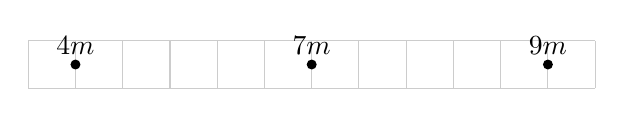
\begin{tikzpicture}[scale=0.6]

\draw[step=1cm,gray!40] (0,0) grid (12,1);

\fill (1,0.5) circle (3pt);
\node[above] at (1,0.5) {$4m$};

\fill (6,0.5) circle (3pt);
\node[above] at (6,0.5) {$7m$};

\fill (11,0.5) circle (3pt);
\node[above] at (11,0.5) {$9m$};

\end{tikzpicture}

\begin{enumerate}[label=\Alph*)]
\item $\dfrac{2Gm^2}{7r^2}$
\item $\dfrac{3Gm^2}{r^2}$
\item $\dfrac{Gm^2}{r^2}$
\item $\dfrac{5Gm^2}{2r^2}$
\end{enumerate}

\item $M$ massali sayyora atrofida $m_0$ va $m$ massali sun’iy yo‘ldoshlar
mos ravishda $3R$ va $5R$ radiusli aylana orbitalar bo‘ylab harakatlanmoqda. Sun’iy yo‘ldoshlarning o‘zaro gravitatsion ta’sir kuchini aniqlang. $\cos\alpha=\frac{3}{5}$

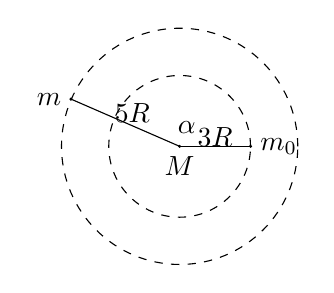
\begin{tikzpicture}[scale=0.3]

\draw[dashed] (0,0) circle (3);
\draw[dashed] (0,0) circle (5);

\fill (0,0) circle (2pt);
\node[below] at (0,0) {$M$};

\fill (3,0) circle (2pt);
\node[right] at (3,0) {$m_0$};

\fill (-4.6,2) circle (2pt);
\node[left] at (-4.6,2) {$m$};

\draw (0,0) -- (3,0);
\draw (0,0) -- (-4.6,2);

\node at (1.5,0.4) {$3R$};
\node at (-2,1.4) {$5R$};
\node at (0.3,0.8) {$\alpha$};

\end{tikzpicture}

\begin{enumerate}[label=\Alph*)]
\item $\gamma\dfrac{m_0m}{16R^2}$
\item $\gamma\dfrac{Mm_0}{16R^2}$
\item $\gamma\dfrac{m_0m}{9R^2}$
\item $\gamma\dfrac{m_0m}{25R^2}$
\item $\gamma\dfrac{m_0m}{5R^2}$
\end{enumerate}


\end{enumerate}

\section{Og‘irlik kuchi}

\begin{enumerate}

\item Massasi 50 kg bo‘lgan, yerda turgan jismga ta’sir etuvchi og‘irlik kuchi qanday (N)? 
$g = 10\ \text{m/s}^2$.

\begin{enumerate}[label=\Alph*)]
\item 500
\item 50
\item 10
\item 5
\item 0.2
\end{enumerate}


\item Vertikal ipga osilgan 10 kg massali jism yerda yotibdi. 
Agar ipning taranglik kuchi 30 N bo‘lsa, jism yerni necha Nyuton kuch bilan bosmoqda? 
$g = 10\ \text{N/kg}$.

\begin{enumerate}[label=\Alph*)]
\item 70
\item 50
\item 40
\item 20
\item 100
\end{enumerate}


\item Massasi va radiusi Yernikidan 3 marta kichik bo‘lgan sayyora sirtida jismning og‘irlik kuchi 
Yer sirtidagidan qanday farq qiladi?

\begin{enumerate}[label=\Alph*)]
\item farq qilmaydi
\item 3 marta kam bo‘ladi
\item 3 marta ko‘p bo‘ladi
\item 9 marta kam bo‘ladi
\item 9 marta ko‘p bo‘ladi
\end{enumerate}


\item Oy radiusi Yer radiusidan 3.6 marta, massasi esa 81 marta kichik. Oy uchun erkin tushish tezlanishini aniqlang $(m/s^2)$. $g_{Yer}=10\ \text{m/s}^2$

\begin{enumerate}[label=\Alph*)]
\item 1.6
\item 1.7
\item 1.8
\item 1.9
\item 2.25
\end{enumerate}


\item Qanday balandlikda jismning og‘irligi Yer sirtidagiga qaraganda 
$n$ marta kichik bo‘ladi?

\begin{enumerate}[label=\Alph*)]
\item $R(n-1)$
\item $R(n+1)$
\item $\dfrac{R}{n-1}$
\item $R-n$
\item $\dfrac{R}{n}$
\end{enumerate}


\item Uch Yer radiusiga teng balandlikda erkin tushish tezlanishi 
Yer sirtidagiga nisbatan qanday bo‘ladi?

\begin{enumerate}[label=\Alph*)]
\item 16 marta katta
\item 4 marta katta
\item 16 marta kichik
\item 4 marta kichik
\item 3 marta kichik
\end{enumerate}


\item Yer sirtidan $R$ ga teng balandlikda jismning og‘irlik kuchi $F$ ga teng. 
Yer sirtidan qanday balandlikda shu jismning og‘irlik kuchi $2F$ ga teng bo‘ladi?



\begin{enumerate}[label=\Alph*)]
\item $2R$
\item $2\sqrt{2}R$
\item $(\sqrt{2}-1)R$
\item $\dfrac{R}{2}$
\item $(\sqrt{2}+1)R$
\end{enumerate}


\item Yer sirtidan qanday balandlikda og‘irlik kuchi 
Yer sirtidagi og‘irlik kuchining $64\%$ ini tashkil qiladi?

\begin{enumerate}[label=\Alph*)]
\item 1600
\item 1400
\item 1700
\item 1650
\item 1500
\end{enumerate}

\end{enumerate}